%------------------------------------------------------------------------------
\section{Experimental Methods}
\label{ch:exp}

The experimental data analysed in this chapter was acquired by Xing Chen, under the supervision of Alexander Thiele at the Institute of Neuroscience, Newcastle University.
The experimental protocol was designed by Xing Chen and Alexander Thiele, and has been described previously (\citealp{Chen2013thesis}; \citealp{Chen2013}; \citealp{Chen2014}). % Had to space manually instead of \citep{Chen2014,Chen2013,Chen2013thesis} due to bug
All procedures were carried out in accordance with the European Communities Council Directive RL 2010/63/EC, the US National Institutes of Health Guidelines for the Care and Use of Animals for Experimental Procedures, and the UK Animals Scientific Procedures Act.
Two male macaque monkeys (\num{5} and \num{14} years of age) were used in this study.


\subsection{Head post implantation}

During an initial surgical operation, a custom-made head post (Peek, Tecapeek) was embedded into a dental acrylic head stage.
Details of the surgical procedures and post-operative care have already been published \citep[see][for details]{Thiele2006}.


\subsection{Stimuli}

Stimuli were displayed on a \ac{CRT} monitor with display dimensions \SI{400x320}{\milli\metre} at a viewing distance of \SI{0.54}{\metre}, with resolution \SI{1280x1024}{px}.
The monitor refresh rate was \SI{85}{Hz} for \ac{M1} and \SI{75}{Hz} for \ac{M2}.


\subsection{Initial training}

The monkeys were familiarised with the experimental set-up and structure with an initial training task otherwise unrelated to the main perceptual learning task on which the animals were later trained.
In this initial task, the animals compared the colour of a circle stimulus with that of succeeding circle stimuli, while maintaining fixation on a central target.
When a target stimulus appeared (a circle of a matching colour), subjects were required to release a touch bar in order to receive a fluid reward.
Eye position was monitored using an infrared video tracking system.% (Dalsa CCD camera, model SIM-0002, and eye-tracking software from Thomas Recording ET-49 --- Version 1.2.8).


\subsection{Electrode array implantation}

During surgery, animals were sedated with ketamine, and general anaesthesia was maintained using isoflurane following endotracheal intubation.
% Heart rate, respiratory rate, blood pressure, \ac{ECG}, \ce{O2} saturation, expiratory \ce{CO2}, and skin and rectal body temperature were monitored continuously during the operation.
% Fluids and antibiotics were administered intravenously.
% The animals were placed in a stereotaxic head holder and the skull overlying the occipital and posterior temporal cortices was exposed.
A craniotomy was made to remove the bone overlying \ac{V1}, \ac{V2}, and dorsal \ac{V4}, using a pneumatic drill.
The bone was kept in sterile $0.9\%$ \ac{NaCl} for refitting at the end of the surgery.
The dura was opened up to allow access to regions \ac{V4} and \ac{V1}.
Microelectrode chronic Utah arrays, attached to a CerePortTM base, were implanted under sterile conditions in the cortex.
%, using a Blackrock microarray inserter.
For \ac{M1}, two $4{\times}5$ grids of microelectrodes were implanted in area \ac{V4}, and one $5{\times}5$ grid was implanted in \ac{V1}.
For \ac{M2}, a $5{\times}5$ grid was implanted in \ac{V4}, and a $5{\times}5$ grid in \ac{V1}.
% The electrode contacts within each \ac{MEA} had a separation distance of XXX, which is sufficiently distant from each other such that neurons can be close enough at most one electrode contact for their spiking activity to be detected.
% Wire bundles were held in place with biologically-compatible glue (histoacrylic), and the connector (CerePortTM) was secured to the skull with titanium bone screws.
% In both animals, the titanium screws were rejected by the bone within 6 to 10 weeks following the implant, so a dental acrylic bridge was built to fuse the base of1 the connector to the existing head stage, during a subsequent surgical operation.

A minority of electrode contacts were unstable, and post-surgery were found to have excessively high impedance.
These electrodes (channels) were not viable for use in electrophyisiological recordings.
The number of recording channels from the \acp{MEA} used in the study are shown in \autoref{tab:nchannels}.

\begin{table}[bthp]
\begin{center}
\begin{tabular}{ccr}
\toprule
Animal   & Region   & Number of viable channels \\
\midrule
\acs{M1} & \acs{V4} & 30 \\
         & \acs{V1} & 23 \\
\acs{M2} & \acs{V4} & 20 \\
         & \acs{V1} & 25 \\
\bottomrule
\end{tabular}
\end{center}
\caption{
\captionemph{Number of channels from which recordings were taken, for each of the monkeys and brain regions.}
}
\label{tab:nchannels}
\end{table}


\subsection{Receptive fields}

After animals had fully recovered, \acp{RF} were mapped using reverse correlation between random visual stimulation and neuronal response.
For both animals, the \acp{RF} of neurons recorded from the \ac{V4} arrays were \SI{7.5}{\degree} from the centre of the visual field.
For \ac{M1}, the \ac{MEA} in \ac{V1} was \SI{4.6}{\degree} from the centre, and for \ac{M2} it was \SI{1.5}{\degree}.
% In macaques, the foveal region spans \SI{\pm1}{\degree} from the centre of vision.
% (Hanazono, Tsunoda, Kazato, Suzuki, & Tanifuji, 2012)

The \ac{RF} locations for the implantation sites in \ac{V4} and \ac{V1} were not retinotopically congruent for either animal.
Consequently, for each animal the experimental protocol was performed first in the peripheral region of the visual field corresponding to the \ac{RF} of the \ac{V4} array, and then repeated in the parafoveal region corresponding to the \ac{V1} array.

Since the improvements in task-performance driven by perceptual learning are known to be specific to stimuli at the same location as the training stimuli (\citealp{Fiorentini1980}; \citealp{Fiorentini1981,Poggio1991,Karni1991}), training the animal on the stimulus at the peripheral location should not impact its performance when the experiment is repeated at a parafoveal location.


\subsection{Behavioural task}
\label{sec:pl_task}

The experimental design has been described previously \citep[see][]{Chen2013}.
Training on the perceptual learning task, whilst recording from the \ac{MEA} implanted in the visual cortex, proceeded over several weeks.
Each day, 5 days per week, the subject had a single recording session composed of multiple trials.
During each trial, the subject is tasked with identifying whether a \termemph{test} stimulus has higher or lower contrast than a preceding \termemph{sample} (or \termemph{pedestal}) stimulus of $30\%$ contrast (\acl{2AFC}, \acsu{2AFC}).
If the subject responds correctly, they are provided with a water reward.
Training continued until the subject's test performance stabilised at a plateau.

Each trial consists of 6 steps, listed below and depicted in \autoref{fig:pltask1}.
\begin{enumerate}
\item The trial begins with the appearance of a \termemph{fixation point}, on which the subject must focus their gaze.
\item A \termemph{sample stimulus} appears in the form of either a Gabor patch (\ac{V4} recordings) or a circular sinusoidal grating (\ac{V1} recordings), presented at the pedestal contrast of $30\%$ in the location corresponding to the \ac{RF} of the \ac{MEA}.
The sample stimulus is presented for approximately \SI{530}{\milli\second}.
\item The fixation target persists, and the sample stimulus disappears.
This period of unstimulated spontaneous neural activity is the \termemph{sample-test interval}, with either fixed or variable duration (see \autoref{tab:tptimes}).
\item A \termemph{test stimulus} appears in the same location as the sample stimulus, but with a different contrast.
The test contrast is selected randomly from a set of \num{14} possibilities (stimulus location dependent, see \autoref{tab:pl_stim}).
This stimulus is presented for approximately \SI{530}{\milli\second}.
\item The fixation target persists, and the test stimulus disappears.
This period of unstimulated spontaneous neural activity is the \termemph{test-target interval}, with duration approximately \SI{425}{\milli\second}.
\item Two \termemph{target stimuli} appear above and to the right of the fixation point (which disappears).
The subject may now make a saccade to their chosen target to indicate whether they think the test stimulus had higher or lower contrast than the sample.
\item If the subject responds correctly, a water reward is dispensed.
\item After a blank inter-trial period, the fixation target reappears and a new trial begins.
\end{enumerate}
All stimuli are presented over a uniform grey background.
The subject must fixate on the central target throughout the sections 1 to 5 of the trial, otherwise the trial is aborted.
Only completed (unaborted) trials were included in the analysis.


\begin{figure}[tbhp]
\begin{center}
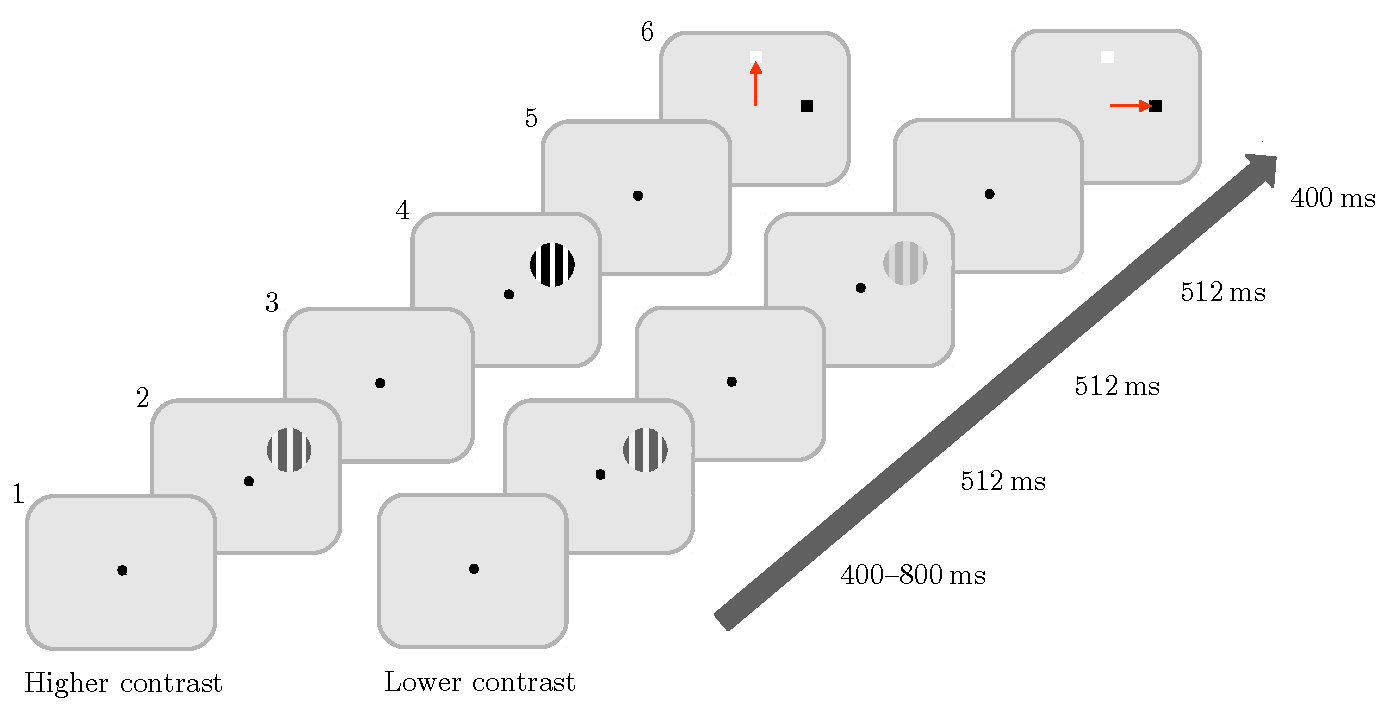
\includegraphics[width=\linewidth]{figs/task/PLtask1.pdf}
\end{center}
\caption{
\captionemph{Experimental procedure.}
1:~The monkey fixates upon a central spot.
2:~A sample stimulus, either a Gabor patch or a sinusoidal grating, is presented with $30\%$ contrast.
3:~Blank sample-test interval.
4:~Test stimulus presented with either higher or lower contrast.
5:~Blank test-target interval.
6:~Two target stimuli appear, and the subject makes a saccade to one to indicate its choice.
Durations indicated are approximate values; see text for details and \autoref{tab:tptimes} for precise timing.
Stimuli contrasts depicted here are not to scale and are for illustrative purposes only.
}
\label{fig:pltask1}
\end{figure}


% \begin{landscape}
\begin{table}[bthp]
\centerline{
%
% \begin{tabular}{ccr}
% \toprule
% Animal   & Region   & Duration (\si{\milli\second}) \\
% \midrule
%          &          & Inter-trial delay \\
% \midrule
% \acs{M1} & \acs{V4} & $530.872 \le t_1 \le 545.526$ \\
%          & \acs{V1} & $525.803 \le t_1 \le 538.983$ \\
% \acs{M2} & \acs{V4} & $526.295 \le t_1 \le 540.641$ \\
%          & \acs{V1} & $525.834 \le t_1 \le 540.702$ \\
% \midrule
%          &          & Sample presentation duration \\
% \midrule
% \acs{M1} & \acs{V4} & $t_2 = 529.275$ \\
%          & \acs{V1} & $t_2 = 529.275$ \\
% \acs{M2} & \acs{V4} & $t_2 = 533.176$ \\
%          & \acs{V1} & $t_2 = 533.176$ \\
% \midrule
%          &          & Post-sample stimulus delay \\
% \midrule
% \acs{M1} & \acs{V4} & $539.720 \le t_3 \le 1058.673$ \\
%          & \acs{V1} & $t_3 = 541.164$ \\
% \acs{M2} & \acs{V4} & $t_3 = 546.632$ \\
%          & \acs{V1} & $t_3 = 546.570$ \\
% \midrule
%          &          & Test presentation duration \\
% \midrule
% \acs{M1} & \acs{V4} & $t_4 = 529.275$ \\
%          & \acs{V1} & $t_4 = 529.275$ \\
% \acs{M2} & \acs{V4} & $t_4 = 533.176$ \\
%          & \acs{V1} & $t_4 = 533.176$ \\
% \midrule
%          &          & Post-test stimulus delay \\
% \midrule
% \acs{M1} & \acs{V4} & $t_5 = 423.475$ \\
%          & \acs{V1} & $t_5 = 423.475$ \\
% \acs{M2} & \acs{V4} & $t_5 = 426.578$ \\
%          & \acs{V1} & $t_5 = 426.640$ \\
% \bottomrule
%
\begin{tabular}{ccccccc}
\toprule
         &          & \multicolumn{5}{c}{Duration (\si{\milli\second})} \\
\cmidrule(l){3-7}
Animal   & Region   & $t_1$            & $t_2$     & $t_3$             & $t_4$     & $t_5$     \\
\midrule
\acs{M1} & \acs{V4} & $[530.9, 545.5]$ & $529.275$ & $[539.7, 1058.7]$ & $529.275$ & $423.475$ \\
         & \acs{V1} & $[525.8, 539.0]$ & $529.275$ & $541.164$         & $529.275$ & $423.475$ \\
\acs{M2} & \acs{V4} & $[526.3, 540.6]$ & $529.275$ & $546.632$         & $533.176$ & $426.578$ \\
         & \acs{V1} & $[525.8, 540.7]$ & $533.176$ & $546.570$         & $533.176$ & $426.640$ \\
\bottomrule
%
\end{tabular}
} % end centerline
\caption{
\captionemph{Precise durations of each section of a single trial.}
The durations are listed for the
pre-sample delay period ($t_1$),
sample presentation ($t_2$),
sample-test interval ($t_3$),
test presentation ($t_4$), and
test-target interval ($t_5$).
Square brackets indicate a range of possible values.
Precise stimulus durations differ for the two animals due to their respective monitor refresh rates.
}
\label{tab:tptimes}
\end{table}
% \end{landscape}


As mentioned in \autoref{sec:bgpl}, previous studies have found it is necessary to present flanking stimuli around the main stimulus in order to induce perceptual learning.
During our experimental study, preliminary research demonstrated flankers were not necessary for perceptual learning provided the contrast of the pedestal stimulus was held the same for every trial.

Trials were presented in blocks, with each block containing a fixed number of repetitions of each test contrast ordered at random.
To ensure the subject was incentivised to attempt all the trials and not just excel at the easiest stimuli, at the end of each block any trials which received incorrect responses were repeated.


\begin{table}[bthp]
\centerline{
\begin{tabular}{cclr}
\toprule
Animal   & Region   & Type      & Test contrasts (\%) \\
\midrule
\acs{M1} & \acs{V4} & Gabor     & 10, 15, 20, 25, 27, 28, 29, 31, 32, 33, 35, 40, 50, 60 \\
         & \acs{V1} & sinusoid  &  5, 10, 15, 20, 22, 25, 28, 32, 35, 40, 45, 50, 60, 90 \\
\acs{M2} & \acs{V4} & Gabor     & 10, 15, 20, 25, 27, 28, 29, 31, 32, 33, 35, 40, 50, 60 \\
         & \acs{V1} & sinusoid  &  5, 10, 15, 20, 22, 25, 28, 32, 35, 40, 45, 50, 60, 90 \\
\bottomrule
%
\end{tabular}
} % end centerline
\caption{
\captionemph{Stimuli parameters for each subject and recording region.}
The set of test contrasts were selected so that the difficulty of the task ranged from easy to very hard.
The test contrasts were set such that \ac{M1} achieved a similar initial accuracy for both peripheral and parafoveal stimuli.
}
\label{tab:pl_stim}
\end{table}


\begin{table}[bthp]
\centerline{
\begin{tabular}{lcccc}
\toprule
                            & \multicolumn{2}{c}{Monkey 1}  & \multicolumn{2}{c}{Monkey 2}  \\
                            \cmidrule(r){2-3}               \cmidrule(l){4-5}
                            & \acs{V4}      & \acs{V1}      & \acs{V4}      & \acs{V1}      \\
\midrule
Number of channels          & 30            & 23            & 20            & 25            \\
Number of sessions          & 30            & 17            & 26            & 22            \\
Stimulus location           & peripheral    & parafoveal    & peripheral    & parafoveal    \\
Centre coords (\acs{dva})   & $(-5, 16)$    & $(-3.5, 3)$   & $(-5, 16)$    & $(-0.7, -1.3)$\\
Size (\acs{dva})            & 16            & 3             & 14            & 0.75          \\
Stimulus type               & Gabor         & sinusoid      & Gabor         & sinusoid      \\
Spatial frequency (\acs{cpd})   & 2         & 2             & 2             & 4             \\
\bottomrule
%
\end{tabular}
} % end centerline
\caption{
\captionemph{Experimental details for each animal and \ac{MEA} recording region.}
Stimulus co-ordinates are given in \acf{dva}.
Spatial frequency is specified in \acf{cpd}.
}
\label{tab:pl_stim2}
\end{table}


The number of trials per recording session was not fixed; the recording session was terminated when the subject was no longer interested in engaging with the experiment.
Consequently there was high variability in the number of trials per session, ranging from \num{254} to \num{1889}.

During training, the subject's performance on the task initially increased each day.
After around \num{20} sessions, its performance stabilised at a plateau.
Once the performance level was consistent for \num{5} consecutive sessions, this phase of the experiment was terminated.

The subject then progressed to a roving version of the experiment, in which the pedestal contrast could be either $20\%$, $30\%$ or $40\%$ contrast.
In the roving task, the subject asked to respond as to whether the test contrast exceeded the variable sample contrast.
However, here we will only analyse the results of the non-roving version of the experiment with a static pedestal contrast of $30\%$.


\subsection{Data acquisition}

Raw data was acquired at a sampling frequency of \SI{32556}{Hz} using a \SI{24}{bit} analog-to-digital converter.
The minimum and maximum inputs were \SI{11}{\micro\volt} and \SI{136986}{\micro\volt} --- values outside this range were recorded at the floor or ceiling value respectively.
To ensure data was collected from each channel with a good signal-to-noise ratio, digital referencing was performed prior to recording the raw data.

Raw data was subsequently bandpass filtered with a lower cutoff frequency of \SI{600}{Hz} and an upper cutoff from within the range \SIrange{2500}{4000}{Hz}.
The upper cutoff frequency was manually selected for each channel and session such that it was low enough to exclude high frequency noise from the experimental equipment, but no lower than necessary.


\subsection{Initial spike extraction}
\label{sec:pl_spike_extraction}

Spikes were extracted from the filtered data using a voltage threshold.
For each recording channel and session, a threshold was selected by hand at a voltage higher than the background noise, such that both high and low amplitude spikes will exceed the threshold.
For each channel, the extracted spike trains contain spikes from multiple neurons (multi-unit activity) surrounding the electrode.
All the spikes from high-amplitude neurons close to the electrode will be included, but lower-amplitude spikes from further away may be detected with a peak voltage around the detection threshold.
Consequently, only a subset of the spikes from more distant neurons will be detected.

After defining a detection threshold, spikes were extracted using the following algorithm.
\begin{enumerate}
\item Find the first sample point to exceed the threshold.
\item Find the peak of the spike by searching for next time the voltage decreases (searching forwards by at most \num{24} data points, spanning \SI{0.74}{\milli\second}).
\item Extract the \num{8} data points preceding and \num{23} data points succeeding the peak as the waveform of the spike, with duration \SI{0.98}{\milli\second}.
\item Skip forward to the end of the extracted waveform (\num{24} data points after the peak) before searching for the next sample point to exceed the threshold again.
\end{enumerate}
By its construction, this algorithm enforces a minimum inter-spike interval of \SI{0.74}{\milli\second}.
